\documentclass{article}
\usepackage[utf8]{inputenc}
\usepackage{hyperref}
\usepackage{multicol}
\setlength{\columnsep}{1cm}
\usepackage[margin=0.5in]{geometry}

\title{Deep Learning Course - Final Project}
\author{Nitsan BenHanoch (208585927), Nir Koren (316443902), Tsvi Tabach (311292304)}
\date{Submitted as a final project report for the DL course, BIU, 2024}

\usepackage{natbib}
\usepackage{graphicx}

\begin{document}

\maketitle

\section{Introduction}

Deep-Learning in healthcare is a hot topic. As deep neural networks become increasingly involved in patient care, these networks must meet several requirements. Such requirements include high precision rate, transparency in their decision-making, and performing effectively even when valuable data is missing.

\subsection{The Dataset}
Kaggle's chest-xray-pneumonia dataset consists of 5,856 lungs X-Ray images of men and children. Each image is labeled either "healthy", "bacterial-infected" or "viral-infected". The data is split between train/set sets. One important issue to note is the classes are not balanced; each set contains a different ratio of images from the different classes.

\subsection{Our Tasks}
In this project, we demonstrate several different deep-learning techniques we learned during the course.

\textbf{Task 1.a. Binary Classification}: we train a CNN on healthy/sick labeled x-ray images of human lungs;

\textbf{Task 1.b. Multiclass classification}: we further improve the CNN to distinguish between bacterial/viral infection;

\textbf{Task 2. Embedding Space:} we apply KNN and t-SNE on embedding vectors we get from the aforementioned networks;

\textbf{Task 3. Anomaly Detection:} having trained on healthy lungs alone, we use auto-encoders to tell if lungs are sick;

\textbf{Task 4. Explainability}: we decipher the model's decision making, e.g. what's important to each layer and neuron.


\subsection{Related Works}
Previous research, such as \href{https://arxiv.org/pdf/1711.05225.pdf}{CheXNet}, study by Rajpurkar et al. (2017), has shown the advantage of using CNN in medical diagnostics. The model proposed in the paper used CNN to output probability of pneumonia with a heat-map localizing the pneumonia areas from chest X-ray images.

\
\begin{multicols}{2}
[
\section{\centering Task 1.a: Binary Classification}
]
\subsection{Solution}
\subsubsection{The Task}
In this task, we treat both bacterial and viral images as
\textit{sick}, and train a model to classify \textit{healthy}/\textit{sick} lungs x-ray.

\subsubsection{General approach}
We use several convolution layers, followed by a few dense layers. It is the field's classic and go-to way to classify images. Furthermore, the limited dataset size (approximately 5K images) posses a serious restriction on the complexity of the network, as overly powerful architectures risk significant over-fitting.

\subsubsection{Design}
Our network's architecture mimics the great: we took inspiration from the VGG networks' architecture (but we didn't transfer weights; more on that later). 

[TODO CHART WILL GO HERE]

The final version of the notebook takes $\sim$30 minutes to run on Kaggle. 

Provide some general information about your code, platform, how long it took you to train it, technical challenges you had, Loss functions, Optimizers, Architecture, and more.

\subsection{Experimental results}
Provide information about your experimental settings. What alternatives did you measure? Make sure this part is clear to understand, provide as much details as possible. Provide results with tables and figures.

\subsection{Discussion}
Provide some final words and summarize what you have found from running the experiments you described above. Provide some high level insights.

Note - your project will be evaluated for aspects, including the technique you selected, the rational of the experiments you decided to run, the insights you learned from this process and more. Remember, for the purpose of this course, the process that you demonstrate is very  important.

\subsection{Code}

Please provide a link to your colab notebook.

\end{multicols}

\
\begin{multicols}{2}
[
\section{\centering Task 1.2: Multiclass Classification}
]
\subsection{Solution}
\subsubsection{General approach}
Describe your preferred approach to solve the problem. what alternatives you plan to try and why. 

\subsubsection{Design}
Provide some general information about your code, platform, how long it took you to train it, technical challenges you had, Loss functions, Optimizers, Architecture, and more.

\subsection{Experimental results}
Provide information about your experimental settings. What alternatives did you measure? Make sure this part is clear to understand, provide as much details as possible. Provide results with tables and figures.

\subsection{Discussion}
Provide some final words and summarize what you have found from running the experiments you described above. Provide some high level insights.

Note - your project will be evaluated for aspects, including the technique you selected, the rational of the experiments you decided to run, the insights you learned from this process and more. Remember, for the purpose of this course, the process that you demonstrate is very  important.

\subsection{Code}

Please provide a link to your colab notebook.

\end{multicols}


\
\begin{multicols}{2}
[
\section{\centering Task 2: Model Embeddings and Visualization}
]
\subsection{Solution}
\subsubsection{General approach}
Describe your preferred approach to solve the problem. what alternatives you plan to try and why. 

\subsubsection{Design}
Provide some general information about your code, platform, how long it took you to train it, technical challenges you had, Loss functions, Optimizers, Architecture, and more.

\subsection{Experimental results}
Provide information about your experimental settings. What alternatives did you measure? Make sure this part is clear to understand, provide as much details as possible. Provide results with tables and figures.

\subsection{Discussion}
Provide some final words and summarize what you have found from running the experiments you described above. Provide some high level insights.

Note - your project will be evaluated for aspects, including the technique you selected, the rational of the experiments you decided to run, the insights you learned from this process and more. Remember, for the purpose of this course, the process that you demonstrate is very  important.

\subsection{Code}

Please provide a link to your colab notebook.

\end{multicols}


\
\begin{multicols}{2}
[
\section{\centering Task 3: Anomaly Detection}
]
\subsection{Solution}
\subsubsection{General approach}
Describe your preferred approach to solve the problem. what alternatives you plan to try and why. 

\subsubsection{Design}
Provide some general information about your code, platform, how long it took you to train it, technical challenges you had, Loss functions, Optimizers, Architecture, and more.

\subsection{Experimental results}
Provide information about your experimental settings. What alternatives did you measure? Make sure this part is clear to understand, provide as much details as possible. Provide results with tables and figures.

\subsection{Discussion}
Provide some final words and summarize what you have found from running the experiments you described above. Provide some high level insights.

Note - your project will be evaluated for aspects, including the technique you selected, the rational of the experiments you decided to run, the insights you learned from this process and more. Remember, for the purpose of this course, the process that you demonstrate is very  important.

\subsection{Code}

Please provide a link to your colab notebook.

\end{multicols}


\
\begin{multicols}{2}
[
\section{\centering Task 4: Explainability in Deep Learning}
]
\subsection{Solution}
\subsubsection{General approach}
Describe your preferred approach to solve the problem. what alternatives you plan to try and why. 

\subsubsection{Design}
Provide some general information about your code, platform, how long it took you to train it, technical challenges you had, Loss functions, Optimizers, Architecture, and more.

\subsection{Experimental results}
Provide information about your experimental settings. What alternatives did you measure? Make sure this part is clear to understand, provide as much details as possible. Provide results with tables and figures.

\subsection{Discussion}
Provide some final words and summarize what you have found from running the experiments you described above. Provide some high level insights.

Note - your project will be evaluated for aspects, including the technique you selected, the rational of the experiments you decided to run, the insights you learned from this process and more. Remember, for the purpose of this course, the process that you demonstrate is very  important.

\subsection{Code}

Please provide a link to your colab notebook.

\end{multicols}

\begin{figure}
  \centering
  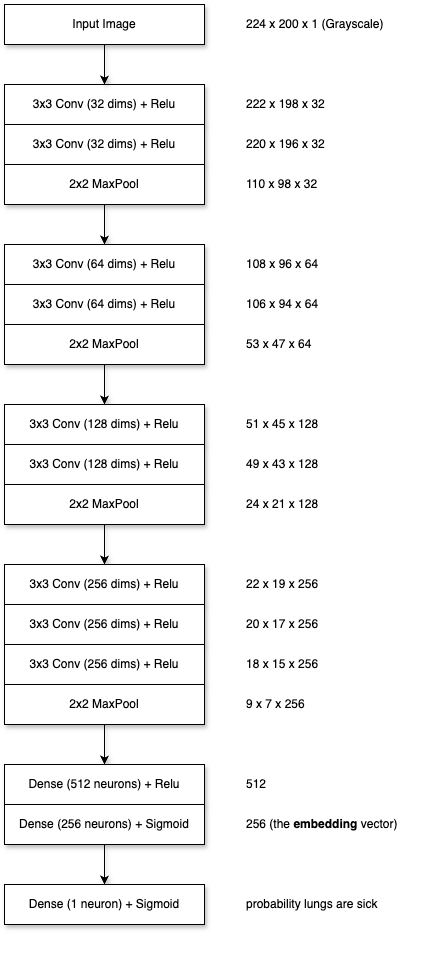
\includegraphics[width=0.45\linewidth]{model_1.png}
  \caption{Binary Classification Model}
  \label{fig:model_1}
\end{figure}


Good luck!!
\bibliographystyle{plain}
\bibliography{references}
\end{document}